\documentclass{sigchi}

% Use this section to set the ACM copyright statement (e.g. for
% preprints).  Consult the conference website for the camera-ready
% copyright statement.

% Copyright
\CopyrightYear{2017}
%\setcopyright{acmcopyright}
\setcopyright{acmlicensed}
%\setcopyright{rightsretained}
%\setcopyright{usgov}
%\setcopyright{usgovmixed}
%\setcopyright{cagov}
%\setcopyright{cagovmixed}
% DOI
\doi{http://dx.doi.org/10.475/123_4}
% ISBN
\isbn{123-4567-24-567/08/06}
%Conference
\conferenceinfo{CHI'16,}{May 07--12, 2016, San Jose, CA, USA}
%Price
\acmPrice{\$15.00}

% Use this command to override the default ACM copyright statement
% (e.g. for preprints).  Consult the conference website for the
% camera-ready copyright statement.

%% HOW TO OVERRIDE THE DEFAULT COPYRIGHT STRIP --
%% Please note you need to make sure the copy for your specific
%% license is used here!
% \toappear{
% Permission to make digital or hard copies of all or part of this work
% for personal or classroom use is granted without fee provided that
% copies are not made or distributed for profit or commercial advantage
% and that copies bear this notice and the full citation on the first
% page. Copyrights for components of this work owned by others than ACM
% must be honored. Abstracting with credit is permitted. To copy
% otherwise, or republish, to post on servers or to redistribute to
% lists, requires prior specific permission and/or a fee. Request
% permissions from \href{mailto:Permissions@acm.org}{Permissions@acm.org}. \\
% \emph{CHI '16},  May 07--12, 2016, San Jose, CA, USA \\
% ACM xxx-x-xxxx-xxxx-x/xx/xx\ldots \$15.00 \\
% DOI: \url{http://dx.doi.org/xx.xxxx/xxxxxxx.xxxxxxx}
% }

% Arabic page numbers for submission.  Remove this line to eliminate
% page numbers for the camera ready copy
% \pagenumbering{arabic}

% Load basic packages
\usepackage{balance}       % to better equalize the last page
\usepackage{graphics}      % for EPS, load graphicx instead 
\usepackage[T1]{fontenc}   % for umlauts and other diaeresis
\usepackage{txfonts}
\usepackage{mathptmx}
\usepackage[pdflang={en-US},pdftex]{hyperref}
\usepackage{color}
\usepackage{booktabs}
\usepackage{textcomp}

% Some optional stuff you might like/need.
\usepackage{microtype}        % Improved Tracking and Kerning
% \usepackage[all]{hypcap}    % Fixes bug in hyperref caption linking
\usepackage{ccicons}          % Cite your images correctly!
% \usepackage[utf8]{inputenc} % for a UTF8 editor only

% If you want to use todo notes, marginpars etc. during creation of
% your draft document, you have to enable the "chi_draft" option for
% the document class. To do this, change the very first line to:
% "\documentclass[chi_draft]{sigchi}". You can then place todo notes
% by using the "\todo{...}"  command. Make sure to disable the draft
% option again before submitting your final document.
\usepackage{todonotes}

% Paper metadata (use plain text, for PDF inclusion and later
% re-using, if desired).  Use \emtpyauthor when submitting for review
% so you remain anonymous.
\def\plaintitle{ExploX - Seminar Project Proposal}
\def\plainauthor{Kevin M\"uller, Marc Rupp, Lukas Strobel, Xueting Li}
\def\emptyauthor{}
\def\plainkeywords{}

% llt: Define a global style for URLs, rather that the default one
\makeatletter
\def\url@leostyle{%
  \@ifundefined{selectfont}{
    \def\UrlFont{\sf}
  }{
    \def\UrlFont{\small\bf\ttfamily}
  }}
\makeatother
\urlstyle{leo}

% To make various LaTeX processors do the right thing with page size.
\def\pprw{8.5in}
\def\pprh{11in}
\special{papersize=\pprw,\pprh}
\setlength{\paperwidth}{\pprw}
\setlength{\paperheight}{\pprh}
\setlength{\pdfpagewidth}{\pprw}
\setlength{\pdfpageheight}{\pprh}

% Make sure hyperref comes last of your loaded packages, to give it a
% fighting chance of not being over-written, since its job is to
% redefine many LaTeX commands.
\definecolor{linkColor}{RGB}{6,125,233}
\hypersetup{%
  pdftitle={\plaintitle},
% Use \plainauthor for final version.
%  pdfauthor={\plainauthor},
  pdfauthor={\emptyauthor},
  pdfkeywords={\plainkeywords},
  pdfdisplaydoctitle=true, % For Accessibility
  bookmarksnumbered,
  pdfstartview={FitH},
  colorlinks,
  citecolor=black,
  filecolor=black,
  linkcolor=black,
  urlcolor=linkColor,
  breaklinks=true,
  hypertexnames=false
}

% create a shortcut to typeset table headings
% \newcommand\tabhead[1]{\small\textbf{#1}}

% End of preamble. Here it comes the document.
\begin{document}

\title{\plaintitle}

\numberofauthors{4}
\author{%
  \alignauthor{Kevin M\"uller\\
    \affaddr{Saarbr\"ucken, Germany}\\
    \email{s9kvmuel@stud.uni-saarland.de}}\\
  \alignauthor{Marc Rupp\\
    \affaddr{Saarbr\"ucken, Germany}\\
    \email{s9mcrupp@stud.uni-saarland.de}}\\
  \alignauthor{Lukas Strobel\\
    \affaddr{St. Ingbert, Germany}\\
    \email{s8lustro@uni-saarland.de}}\\
  \alignauthor{Xueting Li\\
    \affaddr{Saarbr\"ucken, Germany}\\
    \email{ding14552@gmail.com}}\\
}

\maketitle

\begin{abstract}
  In this proposal, we present ExploX, an app that allows for route creation and exploration of less frequented areas.With this we want to enable the user to generate a more holistic image of their living surroundings and allow them to escape their daily routine. \textbf{}
\end{abstract}

\category{H.5.m.}{Information Interfaces and Presentation
  (e.g. HCI)}{Miscellaneous} \category{See
  \url{http://acm.org/about/class/1998/} for the full list of ACM
  classifiers. This section is required.}{}{}

 
 
 \keywords{Route planning;
 Exploration of unfamiliar areas;
 Navigation;
 Ubiquitous Sports technologies; 
 Endurance sports;
 Motivation  }
 
 \begin{comment}
\section{Keywords}
 Route planning;
 Exploration of unfamiliar areas;
 Navigation;
 Ubiquitous Sports technologies; 
 Endurance sports;
 Motivation  
\end{comment}

 \begin{comment}
\section{LATEX STUFF}
\begin{align*} A Formula = \{1,2,4,7\}   \quad Y = \{3,5,6,8,9,11\} \end{align*} and the Relation \begin{align*} \mathcal{R} = \{(a,b) \in  D^2 | a \neq b \wedge c=a+b \; with\; c \in Y \} \end{align*}
A reference \cite{dorr2009gaze}
 \begin{figure}
\centering
  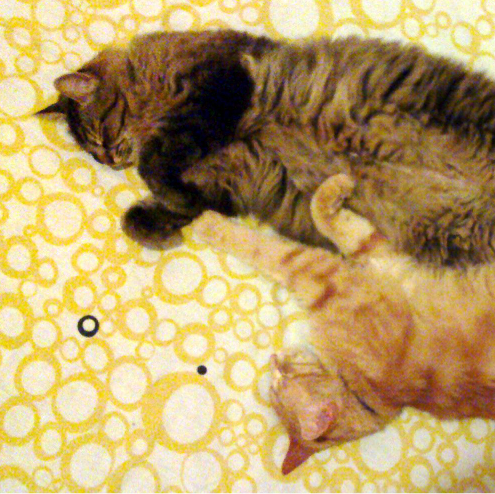
\includegraphics[width=0.2\columnwidth]{figures/cats}
  \caption{This is a sample figure}~\label{fig:figure2}
\end{figure}

\end{comment}


\section{Introduction}
In the last 10 years, the services such as Google Maps that enable point to point navigation and  Geocaching that enable people to explore unfamiliar areas have made great progress and bring more fun. Nowadays also a variety of services such as Strava and Komoot emerge not only navigation but also route planning for running and biking. Based on these services, we want to develop an app which could plan routes and help do personal exploration of the unseen area with the history data using the API of Strava, motivating athletes to cover more less visited parts of their environment.

Our aim here is to motivate athletes to explore more of less visited parts of cities. To accomplish this ,firstly we aim to create routes along paths around areas that the user is most unlikely to know about. The maps would be divided into two parts, the familiar area and unfamiliar area using the history data. The app would recommend person A the routes in seldom visited area but frequent visited by person B, in terms of safety. Secondly our work will allow the user to explore neglected areas knowing the current location and specific destination. So the generated route could be downloaded and preview before exploring. Thirdly, the explored areas would fade out from dark black to transparent according the the frequency of visiting.

Psychogeography is the practice of exploring the urban environment with the intention to investigate the effects on feelings and behavior. To generate a complete image of the city this is necessary, as the Psychogeographers argue. This is one of the  reason we want to create the fading map.

Taking routes of another athlete could avoid the case of illegal exploration or simply routes that are not suited for running or cycling. One has to explore parts of the environment that are normally not frequented.As our aim with this project is not to support illegal activities we do not consider the actual exploration of such areas  which is regarded as danger.

Using the social media sources and personal location history we determine areas that are less frequented and might be unknown even to citizens living in the city for a long time. The design of the ExploX application, tries to combine the ideas of the psychogeography movement from the 60s with more recent developments of the exploration and Strava communities. With this we want to enable the user to generate a more holistic image of their living surroundings and allow them to escape their daily routine. Additionally we hope to complete the users spatial memory about their city.

The paper is structured as follows. First we present the introduction and related work that led to the development of this idea. Afterwards we lay out the designing milestones, a list of equipment and resources we need and the formal requirements for this prototype. Thereafter we will present how we want to conduct the user study in order to evaluate our approach. 

\section{Related Work}
In the following section, we will examine previous work done on the topics of route planning, (urban) exploration and motivation in sports and sightseeing. While the former two topics will give us an overview over different approaches to navigation and goals in exploration, the latter will help us design our prototype in order to motivate users to explore unfamiliar areas as well as complete their training routine and become better athletes.
\subsection{Route Planning}
Route planning has become a very hot research topic in mobile HCI because of the rise of smartphones, smartwatches and other wearables. Pedestrian navigation is particularly interesting because it is much more diverse than the regular turn-by-turn navigation used in car navigation systems.\\
McGookin and Brewster have done an analysis on how runners navigate the environment and presented a novel navigation system for runners \cite{undirectedrunnernav}. Their main finding was that there are two types of running practices. \textit{Familiar location running} is characterized by loops (i.e. circuit tracks). Runners usually plan the route beforehand but only use their mental model of the environment while running. On the other hand, \textit{unfamiliar location running} usually have back runs (i.e. runners go from A to B and then the same way back to A). This is a problem, because unfamiliar location running is mainly used ''as a way to explore the environment and identify places to later visit''. Our approach will address this problem by giving the runners the opportunity to explore new areas and at the same time see as much as possible by not running the same way back again.\\
In order to provide a good running experience, the route has to be selected carefully. There are many approaches that not only use distance and time to calculate a route but also take into account other factors. Stolfi and Alba noticed that most navigators calculated the same route leading to traffic jams \cite{evolutionaryalgonav}. They proposed a system that uses traffic data to re-direct cars in order to spread traffic more evenly, leading to an overall better traffic situation. In particular, they improved travel times by 18\% and greenhouse gas emission by 14\%.\\
Katayama et al. took a similar approach and navigated visitors of events using body-worn sensors in order to avoid congestions and other problems that are difficult for event managers \cite{routeplanningbodywornsensors}.\\
There are web mapping services such as Strava (\hyperlink{http://strava.com}{www.strava.com}) and Komoot (\hyperlink{http://komoot.com}{www.komoot.com}) that also provide information about the surface of the track in order to better plan the route. For instance, cyclists can easily identify off-road streets and plan their route accordingly.\\
As an extension to those online services, Daiber et al. have proposed a concept of \textit{pioneers} to support mountaineers in their route planning. The idea is that users can select a number of friends or experienced mountaineers called \textit{pioneers}. The user will see the routes their pioneers have recently taken and can incorporate them into their own route planning \cite{followthepioneers}. \\


\subsection{Implementation}

\subsection{Evaluation}

\subsection{Conclusion}

\subsection{One paragraph about individual
contribution}

\subsection{Exploration}
As already identified by McGookin and Brewster, exploring the environment is an important motivational factor for runners \cite{undirectedrunnernav}. In familiar location running, the main objectives are to meet a distance, time or place target rather than enjoying the environment. However, when the athlete is in an unfamiliar location, these objectives are reversed. They find that this is mostly the case on holidays, however, we want to find out whether we can get athletes to take unfamiliar routes and explore areas of cities in which they have been living for a longer period of time as well.\\
Robinson et al. have implemented an approach where they encouraged people to explore an area by giving different haptic feedback when they can take alternative routes \cite{ididitmyway}. They could show that people were able to reach their target with only low-resolution haptic feedback and providing users with alternative path awareness is also beneficial.\\
In a similar way, O'Hara could identify discovering and exploring new places as one of the main motivations in geocaching \cite{o2008understanding}. The targets geocachers are looking for are often hidden in special places that are particularly beautiful or abandoned such as old factories or hospitals.\\
There has also been a movement called \textit{urban exploration movement} where people go to and explore abandoned places \cite{urbanexploration}. The growing interest in geocaching and urban exploration shows that people care about the environment they are living in and want to find out more about it. To support this, Quercia et al. have build a system to determine aesthetic qualities of a city \cite{aestheticslondon}. They used this data in a navigation system where users are guided through particularly beautiful, happy or quiet areas.

\subsection{Motivation and Design}
When designing our system, we must not forget about what motives athletes to do sports in the first place. It is our goal to provide a motivating way to explore the city but this alone will probably not suffice to encourage athletes to use our system in their regular training routine. We will try to incorporate several motivational factors into the design of our system.\\
Vallerand et al. have identified three psychological needs which are the reason why people take part in sports \cite{vallerand2007intrinsic}. Those needs are the need for autonomy, competence and relatedness \cite{vallerand1999integrative}. The need for competence is satisfied by giving the athletes regular success and not make them fail all the time. Some competition is good but overall the training climate should be mastery-oriented and not highly competitive. The need for relatedness is satisfied by providing the possibility for athletes to cooperate, share and do activities together. Giving the users some freedom of what they want to do satisfies their need for autonomy \cite{vallerand2007intrinsic}.\\
In a similar fashion, Ross and Iso-Ahola have identified knowledge-seeking and social interaction as the dominating motivation force in sightseeing. The bottom line from their research is that it is important to teach users something while they are exploring and at the same time give them the opportunity for social interaction \cite{DUNNROSS1991226}.

\section{Evaluation \& Testing}
Testing and Evaluation will be a key part of our project. We will split this into three parts. 
\subsection{First Part}
The first part starts in January. Therefore we will find five to ten athletes that participate in our study. If that works we will work together with the triathlon squad here in Saarbr\"ucken. Each athlete will give us the permission to get their tracked Strava activities for research purposes. We collect the data for about ten days or two weeks and want the participants to write a training diary in this time. The advantage with the triathletes would be that they do training frequently also in winter. 
\subsection{Second Part}
The second part of the study will be around February. Then we will tell the participants, which product we are working on and give them admission to our web tool. Now they will do the same thing as before but with our software. This time the goal is to make them familiar with the tool and have them use it. After they had an introduction to the tool the participants start another ten days or two weeks this time using the software and writing diary also concerning the software. 
Our hypothesis is: Athletes will explore new areas using our system than in their regular training routine.
\subsection{Third Part}
The third part will be the evaluation. After our software finally works we can now also calculate the black map that fades away with the gathered data from part one. So we can easily compare the two maps from part one with part two and do this with each athlete. 
To get more feedback we will also conduct semi-structured interviews with them and give them questionnaires of about two pages. Then we can also avoid complications like if an athlete was ill in one of the two parts or had other reasons not to use our software often we can consider this in the evaluation
Then we can see whether the athletes could discover new areas by looking at the two maps and either support or reject our hypothesis.

% BALANCE COLUMNS
\balance{}

% REFERENCES FORMAT
% References must be the same font size as other body text.
\bibliographystyle{SIGCHI-Reference-Format}
\bibliography{sample}

\end{document}

%%% Local Variables:
%%% mode: latex
%%% TeX-master: t
%%% End:
